%%%%%%%%%%%%%%%%%%%%%%%%%%%%%%%%%%%%%%%%%
% Masters/Doctoral Thesis 
% LaTeX Template
% Version 2.5 (27/8/17)
%
% This template was downloaded from:
% http://www.LaTeXTemplates.com
%
% Version 2.x major modifications by:
% Vel (vel@latextemplates.com)
%
% This template is based on a template by:
% Steve Gunn (http://users.ecs.soton.ac.uk/srg/softwaretools/document/templates/)
% Sunil Patel (http://www.sunilpatel.co.uk/thesis-template/)
%
% Template license:
% CC BY-NC-SA 3.0 (http://creativecommons.org/licenses/by-nc-sa/3.0/)
%
%%%%%%%%%%%%%%%%%%%%%%%%%%%%%%%%%%%%%%%%%

%----------------------------------------------------------------------------------------
%	PACKAGES AND OTHER DOCUMENT CONFIGURATIONS
%----------------------------------------------------------------------------------------

\documentclass[
12pt, % The default document font size, options: 10pt, 11pt, 12pt
twoside, % Two side (alternating margins) for binding by default, uncomment to switch to one side
australian, % ngerman for German
onehalfspacing, %singlespacing, % Single line spacing, alternatives: onehalfspacing or doublespacing
%draft, % Uncomment to enable draft mode (no pictures, no links, overfull hboxes indicated)
nolistspacing, % If the document is onehalfspacing or doublespacing, uncomment this to set spacing in lists to single
liststotoc, % Uncomment to add the list of figures/tables/etc to the table of contents
toctotoc, % Uncomment to add the main table of contents to the table of contents
parskip, % Uncomment to add space between paragraphs
%nohyperref, % Uncomment to not load the hyperref package
headsepline, % Uncomment to get a line under the header
chapterinoneline, % Uncomment to place the chapter title next to the number on one line
%consistentlayout, % Uncomment to change the layout of the declaration, abstract and acknowledgements pages to match the default layout
]{MastersDoctoralThesis} % The class file specifying the document structure


% ********************************************************************
% Bibliography commands STARTS
% ********************************************************************

%\usepackage[backend=biber,maxcitenames=2,maxbibnames=9,style=authoryear,natbib=true,indexing=true]{biblatex} % Use the bibtex backend with the authoryear citation style (which resembles APA)

\PassOptionsToPackage{
    	natbib=true,
    	style=authoryear-comp,
    	dashed=false,
    	hyperref=true,
    	backend=biber,
    	%bibencoding=ascii,
    	maxbibnames=10,
    	giveninits=true,
    	uniquename=false,%init,
		uniquelist=false,
    	maxcitenames=2,
    	parentracker=true,
    	%url=true,
    	%urldate=long,
    	%dateabbrev=false,
    	doi=true,
    	isbn=true,
		%eprint=false,
    	backref=false,
    	sorting=nyt,%ynt,%nyt,
    	sortcites=true,
    }   {biblatex}
    \usepackage{biblatex}
  \DeclareNameAlias{sortname}{family-given} 
  
  %Remove quotes from article titles
 % \DeclareFieldFormat[article, inbook, incollection, inproceedings, misc, thesis, unpublished]{title}{#1}
  
    % report either doi (preffered) or url (if no doi)
    \renewbibmacro*{doi+eprint+url}{% 
    \iftoggle{bbx:url} 
    {\iffieldundef{doi}{\usebibmacro{url+urldate}}{}} 
    {}% 
    \newunit\newblock 
    \iftoggle{bbx:eprint} 
    {\usebibmacro{eprint}} 
    {}% 
    \newunit\newblock 
    \iftoggle{bbx:doi}
    {\printfield{doi}}
    {}}
  
  % remove "in:" from articles. Thanks to Herbert.
    \renewbibmacro{in:}{%
    	\ifentrytype{article}{}{%
    		\printtext{\bibstring{in}\intitlepunct}}}
    
    % omit "month" and "language" from Bibliography
    \AtEveryBibitem{%
    	\clearfield{month}{}%
    	\clearlist{language}{}%
    }
    
     % omit from type "articles" from Bibliography
    \AtEveryBibitem{\ifentrytype{article}{\clearfield{issn}\clearfield{isbn}}{}}
    
    % some natbib backwards compatibility 
     \let\citealp\cite
     \let\cite\textcite
    
     % increase vertical space between bibliography items.
     \setlength\bibitemsep{0.5ex}
     \setlength\bibnamesep{1.2ex}
    
    % Comma before and after journal volume. Thanks to lockstep.
    \renewbibmacro*{volume+number+eid}{%
    	\setunit*{\addcomma\space}% NEW
    	\printfield{volume}%
    	\printfield{number}%
    	\printfield{eid}}
    \DeclareFieldFormat[article]{number}{(#1)}% number of a journal
    
    % Citation Hyperlinks (not just years), thanks to Audrey.
    \makeatletter
    \renewbibmacro*{cite}{% Based on cite bib macro from authoryear-comp.cbx
    	\iffieldundef{shorthand}
    	{\ifthenelse{\ifnameundef{labelname}\OR\iffieldundef{labelyear}}
    		{\printtext[bibhyperref]{% Include labelname in hyperlink
    				\DeclareFieldAlias{bibhyperref}{default}% Prevent nested hyperlinks
    				\usebibmacro{cite:label}%
    				\setunit{\addspace}%
    				\usebibmacro{cite:labeldate+extradate}}%
    			\usebibmacro{cite:reinit}}
    		{\iffieldequals{namehash}{\cbx@lasthash}
    			{\ifthenelse{\iffieldequals{labelyear}{\cbx@lastyear}\AND
    					\(\value{multicitecount}=0\OR\iffieldundef{postnote}\)}
    				{\setunit{\addcomma}%
    					\usebibmacro{cite:extradate}}
    				{\setunit{\compcitedelim}%
    					\usebibmacro{cite:labeldate+extradate}%
    					\savefield{labelyear}{\cbx@lastyear}}}
    			{\printtext[bibhyperref]{% Include labelname in hyperlink
    					\DeclareFieldAlias{bibhyperref}{default}% Prevent nested hyperlinks
    					\printnames{labelname}%
    					\setunit{\nameyeardelim}%
    					\usebibmacro{cite:labeldate+extradate}}%
    				\savefield{namehash}{\cbx@lasthash}%
    				\savefield{labelyear}{\cbx@lastyear}}}}
    	{\usebibmacro{cite:shorthand}%
    		\usebibmacro{cite:reinit}}%
    	\setunit{\multicitedelim}}
    
    \renewbibmacro*{textcite}{% Based on textcite bib macro from authoryear-comp.cbx
    	\iffieldequals{namehash}{\cbx@lasthash}
    	{\iffieldundef{shorthand}
    		{\ifthenelse{\iffieldequals{labelyear}{\cbx@lastyear}\AND
    				\(\value{multicitecount}=0\OR\iffieldundef{postnote}\)}
    			{\setunit{\addcomma}%
    				\usebibmacro{cite:extradate}}
    			{\setunit{\compcitedelim}%
    				\usebibmacro{cite:labeldate+extradate}%
    				\savefield{labelyear}{\cbx@lastyear}}}
    		{\setunit{\compcitedelim}%
    			\usebibmacro{cite:shorthand}%
    			\global\undef\cbx@lastyear}}
    	{\ifnameundef{labelname}
    		{\printtext[bibhyperref]{% Include labelname in hyperlink
    				\DeclareFieldAlias{bibhyperref}{default}% Prevent nested hyperlinks
    				\iffieldundef{shorthand}
    				{\usebibmacro{cite:label}%
    					\setunit{%
    						\global\booltrue{cbx:parens}%
    						\addspace\bibopenparen}%
    					\ifnumequal{\value{citecount}}{1}
    					{\usebibmacro{prenote}}
    					{}%
    					\usebibmacro{cite:labeldate+extradate}}
    				{\usebibmacro{cite:shorthand}}%
    				\ifthenelse{\iffieldundef{postnote}\AND
    					\(\value{multicitetotal}=0\AND\value{citetotal}=1\)}
    				{\bibcloseparen% Include closing parenthesis in hyperlink
    					\global\boolfalse{cbx:parens}}
    				{}}}
    		{\printtext[bibhyperref]{% Include labelname in hyperlink
    				\DeclareFieldAlias{bibhyperref}{default}% Prevent nested hyperlinks
    				\printnames{labelname}%
    				\setunit{%
    					\global\booltrue{cbx:parens}%
    					\addspace\bibopenparen}%
    				\ifnumequal{\value{citecount}}{1}
    				{\usebibmacro{prenote}}
    				{}%
    				\iffieldundef{shorthand}
    				{\iffieldundef{labelyear}
    					{\usebibmacro{cite:label}}
    					{\usebibmacro{cite:labeldate+extradate}}%
    					\savefield{labelyear}{\cbx@lastyear}}
    				{\usebibmacro{cite:shorthand}%
    					\global\undef\cbx@lastyear}%
    				\ifthenelse{\iffieldundef{postnote}\AND
    					\(\value{multicitetotal}=0\AND\value{citetotal}=1\)}
    				{\bibcloseparen% Include closing parenthesis in hyperlink
    					\global\boolfalse{cbx:parens}}
    				{}}%
    			\savefield{namehash}{\cbx@lasthash}}}%
    	\setunit{%
    		\ifbool{cbx:parens}
    		{\bibcloseparen\global\boolfalse{cbx:parens}}
    		{}%
    		\multicitedelim}}
    \makeatother
    
    % Backrefs "cited" instead of "cit"
    \DefineBibliographyStrings{english}{%
    	backrefpage={cited on p\adddot},
    	backrefpages={cited on pp\adddot}
    }
        

% ********************************************************************
% Bibliography commands ENDS
% ********************************************************************
%\DeclareFieldFormat{url}{\mkbibacro{URL}\addcolon\space\href{#1}{\faExternalLink}}
\DeclareFieldFormat{url}{\href{#1}{\faExternalLink}}
    
\addbibresource{SW-biblatex.bib} % The filename of the bibliography
%\addbibresource{references.bib} % The filename of the bibliography %Bibliography commands


% ********************************************************************
% Useful commands
% ********************************************************************
\newcommand{\ie}{i.\,e.~}
\newcommand{\Ie}{I.\,e.~}
\newcommand{\eg}{e.\,g.~}
\newcommand{\Eg}{E.\,g.~}

%----------------------------------------------------------------------------------------

% Define some commands to keep the formatting separated from the content 
\newcommand{\keyword}[1]{\textbf{#1}}
\newcommand{\tabhead}[1]{\textbf{#1}}
\newcommand{\code}[1]{\texttt{#1}}
\newcommand{\file}[1]{\texttt{\bfseries#1}}
\newcommand{\option}[1]{\texttt{\itshape#1}}
%----------------------------------------------------------------------------------------

%----------------------------------------------------------------------------------------
%	Optional Packages
%----------------------------------------------------------------------------------------
\usepackage{graphicx}
\usepackage[figuresright]{rotating}
\usepackage[utf8]{inputenc} % Required for inputting international characters
\usepackage[T1]{fontenc} % Output font encoding for international characters
%\usepackage{mathpazo} % Use the Palatino font by default
\usepackage{mathptmx} % Sheng prefer font close to New Roman
%\usepackage{tgpagella} %The TEX Gyre Pagella family of fonts is based on the URW Palladio family, but heavily extended (https://www.tug.org/FontCatalogue/texgyrepagella/)

\usepackage{fontawesome} % Use for loading symbol for URLs
\usepackage{textcomp} % use for degree symbol (\textdegree)
\usepackage{pdfpages}
%\usepackage[document]{ragged2e}

\usepackage{pdftexcmds}
\usepackage[section]{minted} %works well in Overleaf but offline may need Python package to be installed and shell escape setting applied
\usemintedstyle{friendly}
\usemintedstyle{borland}

\usepackage[autostyle=true]{csquotes} % Required to generate language-dependent quotes in the bibliography
\usepackage[font={itshape,raggedright},begintext=``,endtext="]{quoting}
\usepackage{microtype}
\usepackage[framemethod=TikZ]{mdframed}
\usepackage{amssymb}
\usepackage{multirow}
\usepackage{tabulary}
\usepackage{glossaries}
\usepackage{textcomp}

% Sheng
\DeclareUnicodeCharacter{1EA1}{\d{a}} % Sheng
\newcommand{\SORTCITATION}[1]{}
%The following allow display of equations with better presentation -----
\usepackage[retainorgcmds]{IEEEtrantools}
\usepackage[titles]{tocloft}

\newcommand{\listequationsname}{List of Equations}
\newlistof{myequations}{equ}{\listequationsname}
\newcommand{\myequations}[1]{%
\addcontentsline{equ}{myequations}{\protect\numberline{\theequation}#1}\par}
\setlength{\cftmyequationsnumwidth}{2.5em}% Width of equation number in List of Equations

\usepackage{amsmath,bm}

\newcommand{\minus}{\scalebox{0.75}[1.0]{$-$}}
% End of Sheng's revisions

%New colors defined below
\definecolor{LightGray}{gray}{0.9}
\definecolor{codegreen}{rgb}{0,0.6,0}
\definecolor{codegray}{rgb}{0.5,0.5,0.5}
\definecolor{codepurple}{rgb}{0.58,0,0.82}
\definecolor{backcolour}{rgb}{0.95,0.95,0.92}
\definecolor{mintedbackground}{rgb}{0.95,0.95,0.95}
\definecolor{revblue}{rgb}{0.15,0.48,1.0}
\definecolor{revlightblue}{rgb}{0.73,0.83, 0.99}
\definecolor{revred}{rgb}{0.82,0.20,0.22}
\definecolor{revlightred}{rgb}{0.99,0.76,0.77}

%\usepackage{subcaption} %for sub figures

\usepackage{fixme} %FixMe package
\fxsetup{status=draft,author=} % <====== add this line
\fxsetup{theme=color}
\fxsetface{margin}{\scriptsize}
%\definecolor{fxnote}{rgb}{0.0000,0.0000,0.0000}
%\definecolor{fxwarning}{rgb}{0.0000,0.0000,0.0000}
%\definecolor{fxerror}{rgb}{0.0000,0.0000,0.0000}
%\definecolor{fxfatal}{rgb}{0.0000,0.0000,0.0000}

\pdfcompresslevel=9 %best compression
\pdfadjustspacing=1 %for small font expansion

%\usepackage{chngcntr}
%\counterwithin{figure}{section}

%\usepackage[titles]{tocloft}
%\setlength{\cftbeforechapskip}{5pt} \ sets spacing in Table of Contents
% or see http://www-h.eng.cam.ac.uk/help/tpl/textprocessing/squeeze.html

%----------------------------------------------------------------------------------------
%	BOX SETTINGS
%----------------------------------------------------------------------------------------
% from https://texblog.org/2015/09/30/fancy-boxes-for-theorem-lemma-and-proof-with-mdframed/

%Proof
\newcounter{prf}[section]\setcounter{prf}{0}
\renewcommand{\theprf}{\arabic{chapter}.\arabic{section}.\arabic{prf}}
\newenvironment{prf}[2][]{%
\refstepcounter{prf}%
\ifstrempty{#1}%
{\mdfsetup{%
frametitle={%
\tikz[baseline=(current bounding box.east),outer sep=0pt]
\node[anchor=east,rectangle,fill=red!20]
{\strut Proof~\theprf};}}
}%
{\mdfsetup{%
frametitle={%
\tikz[baseline=(current bounding box.east),outer sep=0pt]
\node[anchor=east,rectangle,fill=red!20]
{\strut Box~\theprf:~#1};}}%
}%
\mdfsetup{innertopmargin=10pt,linecolor=red!20,%
linewidth=2pt,topline=true,%
frametitleaboveskip=\dimexpr-\ht\strutbox\relax
}
\begin{mdframed}[]\relax%
\label{#2}}{\end{mdframed}}
%%%%%%%%%%%%%%%%%%%%%%%%%%%%%%


%----------------------------------------------------------------------------------------
%	MARGIN SETTINGS
%----------------------------------------------------------------------------------------

\geometry{
	paper=a4paper, % Change to letterpaper for US letter
	inner=2.5cm, % Inner margin
	outer=2.5cm, % Outer margin
	bindingoffset=.5cm, % Binding offset
	top=1.5cm, % Top margin
	bottom=1.5cm, % Bottom margin
	%showframe, % Uncomment to show how the type block is set on the page
}


%----------------------------------------------------------------------------------------
%	Commands for revising the thesis
%   by Sheng Wang
%----------------------------------------------------------------------------------------
\usepackage{soul}

% command to add
\newcommand{\revadd}[1]{{\color{revred} {#1}}}
%\newcommand{\revadd}[1]{#1}

% command to delete something
\newcommand{\revdel}[1]{{\color{revred} \st{#1}}}
%\newcommand{\revdel}[1]{}


% command to add margin comments
\usepackage[textwidth=1.7cm]{todonotes}
\setlength{\marginparwidth}{2.1cm}
\newcommand{\revcom}[1]{\todo[bordercolor=revlightred,linecolor=revlightred,backgroundcolor=revlightred,size=\scriptsize]{#1}}
%\newcommand{\revcom}[1]{}

% linenumbers
\usepackage{lineno}
\renewcommand\linenumberfont{\normalfont\tiny}
\newcommand{\setlinenumbersheng}{\linenumbers}
%\newcommand{\setlinenumbersheng}{}

%----------------------------------------------------------------------------------------
%	THESIS INFORMATION
%----------------------------------------------------------------------------------------

\thesistitle{Seismic Event Coda-Correlation Imaging of the Earth's Interior} % Your thesis title, this is used in the title and abstract, print it elsewhere with \ttitle
\supervisor{Hrvoje Tkalčić} % Your supervisor's name, this is used in the title page, print it elsewhere with \supname
\examiner{} % Your examiner's name, this is not currently used anywhere in the template, print it elsewhere with \examname
\degree{Doctor of Philosophy} % Your degree name, this is used in the title page and abstract, print it elsewhere with \degreename
\author{Sheng Wang} % Your name, this is used in the title page and abstract, print it elsewhere with \authorname
\addresses{} % Your address, this is not currently used anywhere in the template, print it elsewhere with \addressname
\subject{Geophysics} % Your subject area, this is not currently used anywhere in the template, print it elsewhere with \subjectname
\keywords{} % Keywords for your thesis, this is not currently used anywhere in the template, print it elsewhere with \keywordnames
\university{The Australian National University} % Your university's name and URL, this is used in the title page and abstract, print it elsewhere with \univname
\department{Research School of Earth Sciences} % Your department's name and URL, this is used in the title page and abstract, print it elsewhere with \deptname
\group{} % Your research group's name and URL, this is used in the title page, print it elsewhere with \groupname
\faculty{} % Your faculty's name and URL, this is used in the title page and abstract, print it elsewhere with \facname

\AtBeginDocument{
\hypersetup{pdftitle=\ttitle} % Set the PDF's title to your title
\hypersetup{pdfauthor=\authorname} % Set the PDF's author to your name
\hypersetup{pdfkeywords=\keywordnames} % Set the PDF's keywords to your keywords
}

% Sheng
\setlength{\parskip}{1.0em}

\begin{document}


\frontmatter % Use roman page numbering style (i, ii, iii, iv...) for the pre-content pages

\pagestyle{plain} % Default to the plain heading style until the thesis style is called for the body content

%----------------------------------------------------------------------------------------
%	TITLE PAGE
%----------------------------------------------------------------------------------------

\begin{titlepage}
\begin{center}

\vspace*{0.16\textheight}
%{\scshape\LARGE \univname\par}\vspace{1.5cm} % University name
% \bigskip  
%\textsc{\Large Doctoral Thesis}\\[0.5cm] % Thesis type

%\HRule \\[0.4cm] % Horizontal line

%{\huge \bfseries \ttitle\par}\vspace{0.6cm} % Thesis title automatic

{\bfseries
\LARGE{Seismic Event Coda-Correlation Imaging of the Earth's Interior}\\
%\bigskip
%\large{Astrophysical, Geochemical and Biological Constraints on Habitability}
}

\vspace{1cm} % Thesis title

%\HRule \\[1.2cm] % Horizontal line
 
\begin{minipage}[t]{0.3\textwidth}
\begin{center}
 \large
%\emph{Author:}\\
 \authorname % Author name - remove the \href bracket to remove the link
\end{center}
\end{minipage}

%\begin{minipage}[t]{0.4\textwidth}
%\begin{flushright} \large
%\emph{Supervisor:} \\
%\href{http://www.jamessmith.com}{\supname} % Supervisor name - remove the \href bracket to remove the link  
%\end{flushright}
%\end{minipage}\\[3cm]

\vspace{6.3cm}
%\vspace{1cm}
%\includegraphics[width=0.6\textwidth]{gfx/front_cover.pdf} \\ \bigskip  
%\vspace{1cm}

\large \textit{A thesis submitted for the degree of \degreename}\\[0.7cm] % University requirement text

\vspace{0.0cm}

%\textit{in the}\\[0.4cm]
\groupname

\deptname % Research group name and department name

\vspace{-0.3cm}

\univname % University name

%{\small Draft (\today)}\\[2cm] % Date
%\includegraphics{Logo} % University/department logo - uncomment to place it


\includegraphics[width=6cm]{gfx/ANU_LOGO_cmyk_56mm.pdf}

\vspace{-0.6cm}

{\normalsize March, 2022}\\[2cm] % Date

\end{center}
\end{titlepage}

%----------------------------------------------------------------------------------------
%	DECLARATION PAGE
%----------------------------------------------------------------------------------------

\begin{declaration}
%\addchaptertocentry{\authorshipname} % Add the declaration to the table of contents
\begingroup
\large
\noindent This thesis presents a collection of research works conducted between May 2018 and February 2022 at the Research School of Earth Sciences, The Australian National University, Canberra, Australia. Except where acknowledged in the text, the material presented in this thesis is, to the best of my knowledge, original and has not been submitted in whole or part for a degree in any university. Co-authors have given formal consent for all papers to be presented in this thesis.
%\begin{itemize}
%\item Chapter~\ref{ch:HabitableWorlds} is the paper \cite{Lineweaver2012AnnRev}. Section~\ref{sec:HZones} is my major research contribution to the paper. Research on the distribution of biomass on Earth, the constraints for habitable zones within the Earth, and the energy requirements and sources for the earliest bacteria is my work.
%\item Chapter~\ref{ch:biologicalhab} is the paper \cite{Chopra2016} where my research forms a major contribution to all sections of the paper.
%\end{itemize}


\bigskip
\vspace{1cm}
\begin{flushright}
\authorname\\
\today
\end{flushright}
\endgroup
\end{declaration}
\vspace{3cm}
\begingroup
\endgroup
\cleardoublepage

% \begin{declaration}
% \addchaptertocentry{\authorshipname} % Add the declaration to the table of contents
% \noindent I, \authorname, declare that this thesis titled, \enquote{\ttitle} and the work presented in it are my own. I confirm that:

% \begin{itemize} 
% \item This work was done wholly or mainly while in candidature for a research degree at this University.
% \item Where any part of this thesis has previously been submitted for a degree or any other qualification at this University or any other institution, this has been clearly stated.
% \item Where I have consulted the published work of others, this is always clearly attributed.
% \item Where I have quoted from the work of others, the source is always given. With the exception of such quotations, this thesis is entirely my own work.
% \item I have acknowledged all main sources of help.
% \item Where the thesis is based on work done by myself jointly with others, I have made clear exactly what was done by others and what I have contributed myself.\\
% \end{itemize}
 
% \noindent Signed:\\
% \rule[0.5em]{25em}{0.5pt} % This prints a line for the signature
 
% \noindent Date:\\
% \rule[0.5em]{25em}{0.5pt} % This prints a line to write the date
% \end{declaration}

% \cleardoublepage

%----------------------------------------------------------------------------------------
%	QUOTATION PAGE
%----------------------------------------------------------------------------------------

% \vspace*{0.2\textheight}

% \noindent\enquote{\itshape Thanks to my solid academic training, today I can write hundreds of words on virtually any topic without possessing a shred of information, which is how I got a good job in journalism.}

% \hfill Dave Barry

%----------------------------------------------------------------------------------------
%	ACKNOWLEDGEMENTS
%----------------------------------------------------------------------------------------

\begin{acknowledgements}
\addchaptertocentry{\acknowledgementname} % Add the acknowledgements to the table of contents
\vspace{0.4cm}
\begingroup
\normalsize
Many years later, as looking back, I will still remember the picture of a sunny and warm autumn afternoon when golden leaves fall quietly outside the window, and Hrvoje on the other side of an old desk asked me, ``\textit{...do you accept the challenge...}''. A challenging but fascinating journey with Prof. Hrvoje Tkalčić, my supervisor, began that afternoon. Hrvoje provides me with meticulous academic guidance and helps throughout my PhD progress for tackling the coda-correlation tomography problem. On the other hand, he always inspires me to ``\textit{think big}'', for so many times when I was immersed and deeply captured in a one-track mind. In this journey, I have learned a lot from him. The picture will be in my mind forever. Thank you, Hrvoje!

I am also grateful to Prof. Ian Jackson, Dr Caroline M. Eakin, and Dr Andrew Valentine in my supervisory panel. They always help me reflect on what I have been doing along with my PhD progress. Their insightful comments and suggestions are always beneficial and helpful for completing this thesis. Talking with them can be like finding simple and quick answers on Google, or more often like being immersed in the great ocean of knowledge. Thank you, my supervisory panelists!

I feel lucky and glad to be a part of the Geophysics group (the former Seismology and Mathematical Geophysics group) at the Research School of Earth Sciences (RSES). It is a great environment for learning, research, conversations or debates, and more. It is also a wonderful scene beyond the ivory tower, where I get trained, improved, and connected to the scientific community and real-world sciences. Moreover, the RSES is a warm place to meet friends to share joys and sorrows, with many pictures painted in my mind and never fade!

I am also grateful to the resources and technical support from the National Computational Infrastructure (NCI) and the Terrawulf facility at the RSES for completing this thesis. The Australian Government provides the NCI infrastructure through the National Collaborative Research Infrastructure Strategy scheme (NCRIS). The Terrawulf is developed with support from AuScope, Australia's lead provider of research infrastructure, and funded through the NCRIS.

Finally, I would like to thank my parents, sister, and grandparents. Across a broad ocean, their support and encouragement are always with me!
\endgroup
\end{acknowledgements}



%----------------------------------------------------------------------------------------
%	ABSTRACT PAGE
%----------------------------------------------------------------------------------------

\begin{abstract}
\addchaptertocentry{\abstractname} % Add the abstract to the table of contents
\begingroup
\normalsize
Seismic coda waves are the late part of the seismic energy generated by earthquakes. Global coda correlograms are constructed by cross-correlating and stacking seismic event late coda records that are noisy and seemingly useless, but they exhibit many prominent features sensitive to the Earth's internal structure. Thus, the coda correlation rises as a new paradigm in global observational seismology. As a new category of observation, the correlation features, if interpreted correctly, can provide new information about the Earth's interior.

How to accurately utilise seismic event coda correlations, for instance, in “global coda correlation tomography,” has been controversial and unresolved. Some attempts treat coda correlations as reconstructed seismic waves, which is on a par with methods developed in ambient-noise correlations, for they share similar data processing and computation routines. However, that introduces erroneous interpretation because theoretical analyses have demonstrated fundamental differences in the formation mechanisms of coda correlations and ambient-noise correlations. Therefore, we need a solution, a correct approach, to allow us to use a massive amount of coda correlation observables to increase constraints on the Earth's interior.

This thesis consists of theoretical analyses, method developments, and applications for utilising seismic event coda correlations to image the Earth's interior. We first conduct comprehensive analyses to quantitatively `dissect' coda correlations for their formation mechanism. The analyses reveal the mathematical relationship between coda correlations and the Earth's internal structure. Based on that, we build a novel framework toward global coda correlation tomography. We verify the new framework in experiments and compare it with the method based on the assumption of seismic wave reconstruction. We illustrate significant inaccuracy in tomographic images can arise if coda correlations are treated as reconstructed seismic waves. Then, in an application, we provide a new class of observation for inner-core shear-wave anisotropy utilizing coda correlations in the new framework. We find that inner-core shear waves travel faster by at least ~5 s in directions oblique to the Earth's rotation axis than directions parallel to the equatorial plane (anisotropy of >0.8\%). Our inner-core shear-wave anisotropy observations place new constraints on the inner core mineral composition. Finally, we extend the principles to cross-correlations between source events and devise a new way to build global inter-source correlations. We demonstrate that a single seismic station is sufficient to construct a global correlogram. The correlogram exhibits prominent features sensitive to the internal planetary structures. We show implementations to constrain the Earth's and Martian cores' sizes and confirm a large Martian core. This provides a new paradigm for imaging planetary interiors on a global scale with currently realizable resources in planetary missions.
\bigskip

%\textbf{Keywords:} \keywordnames

\endgroup
\end{abstract}

%----------------------------------------------------------------------------------------
%	LIST OF CONTENTS/FIGURES/TABLES/Equations PAGES
%----------------------------------------------------------------------------------------

\renewcommand{\listfigurename}{List of Figures}
\renewcommand{\listtablename}{List of Tables}

\begin{spacing}{0.94} 
\tableofcontents % Prints the main table of contents
\end{spacing}

\listoffigures % Prints the list of figures
\listoftables % Prints the list of tables
% \listoflistings % Prints the list of python codes

% Sheng
%\makeatletter
\listofmyequations %Write out the List of Equations
\addcontentsline{toc}{chapter}{\listequationsname}
%\makeatother

%----------------------------------------------------------------------------------------
%	ABBREVIATIONS
%----------------------------------------------------------------------------------------

%\begin{abbreviations}{ll} % Include a list of abbreviations (a table of two columns)
%\textbf{ANU}&\textbf{A}ustralian \textbf{N}ational \textbf{U}niversity\\
%\textbf{RSES}&\textbf{R}esearch \textbf{S}chool of \textbf{E}arth \textbf{S}ciences\\
%\end{abbreviations}

%%----------------------------------------------------------------------------------------
%%	PHYSICAL CONSTANTS/OTHER DEFINITIONS
%%----------------------------------------------------------------------------------------
%
%\begin{constants}{lr@{${}={}$}l} % The list of physical constants is a three column table
%
%% The \SI{}{} command is provided by the siunitx package, see its documentation for instructions on how to use it
%
%Speed of Light & $c_{0}$ & \SI{2.99792458e8}{\meter\per\second} (exact)\\
%%Constant Name & $Symbol$ & $Constant Value$ with units\\
%
%\end{constants}

%%----------------------------------------------------------------------------------------
%%	SYMBOLS
%%----------------------------------------------------------------------------------------
%
%\begin{symbols}{lll} % Include a list of Symbols (a three column table)
%
%$a$ & distance & \si{\meter} \\
%$P$ & power & \si{\watt} (\si{\joule\per\second}) \\
%%Symbol & Name & Unit \\
%
%\addlinespace % Gap to separate the Roman symbols from the Greek
%
%$\omega$ & angular frequency & \si{\radian} \\
%
%\end{symbols}

%----------------------------------------------------------------------------------------
%	DEDICATION
%----------------------------------------------------------------------------------------

%\dedicatory{For/Dedicated to/To my\ldots} 




%----------------------------------------------------------------------------------------
%	Statement of contributions
%----------------------------------------------------------------------------------------
\clearpage\null\newpage

\includepdf[pages={1-2}]{-Statement-of-Contributions-Merged.pdf}

%----------------------------------------------------------------------------------------
%	THESIS CONTENT - CHAPTERS
%----------------------------------------------------------------------------------------

\mainmatter % Begin numeric (1,2,3...) page numbering

\pagestyle{thesis} % Return the page headers back to the "thesis" style

% Include the chapters of the thesis as separate files from the Chapters folder
% Uncomment the lines as you write the chapters

\setlinenumbersheng

\chapter{Introduction}\label{ch:intro}

\section{Background and Motivation}\label{sec:intro_background}


Global seismology has come a long way in exploring and understanding the structure and dynamics of the Earth's interior. Powered by numerous forward and inverse techniques, seismological studies on a global scale established a one-dimensional radial structure of the Earth's interior that featured discontinuities and distinct spherical shells: the crust, mantle, outer core (OC), inner core (IC), and most recently, the innermost inner core \citep{dziewonski_preliminary_1981,kennett_constraints_1995,ishii_innermost_2002}. These shells are evidence of the Earth's and planetary differentiation processes \citep{carlson_mechanisms_1994,walter_early_2004}. \revadd{For example, the core existence reveals the segregation process of an iron-rich core from a silicate mantle which is one of the most formative events that sets the conditions for the entire evolution that follows \citep{olson_core_2022,wood_accretion_2006}. Also, the core plays an active role in fundamental processes. On the Earth, the coupling between its OC and IC through the transfer of material and heat actively affects the generation and variations of the geomagnetic field \citep[e.g.,][]{braginsky_structure_1963,buffett_thermal_1996,hollerbach_influence_1993,roberts_geomagnetic_2008}, dynamics of the lowermost mantle \citep[e.g.,][]{aubert_thermochemical_2008,gubbins_melting_2011}, and even processes at Earth's free surface \citep[e.g.,][]{biggin_palaeomagnetic_2015}. On Mars, a relatively large Martian core enriched with light elements, detected by seismic observations, could explain why the red planet lost its magnetic field \citep[e.g.,][]{stahler_seismic_2021,yokoo_stratification_2022}.} In more recent times, three-dimensional models of the Earth \citep{dziewonski_mapping_1984,van_der_hilst_evidence_1997} and their further refinements helped confirm and establish a whole range of structures, such as the mantle transition zone \citep{ritsema_global_2004}, the subducted slabs \citep{widiyantoro_structure_1996}, and large-scale heterogeneities at the base of the mantle \citep{garnero_structure_2008}.\revcom{Revised in response to comment \#3 of of The Associate Dean and the Delegated Authority, and comments \#2 and \#10 of Examiner \#3.}



In the last two decades, the discovery of long-range cross-correlations in the seismic wavefield has allowed for significant advancement in detailed imaging of Earth's subsurface \citep[e.g.,][]{campillo_long-range_2003,shapiro_high-resolution_2005}. In the ambient noise wavefield, the cross-correlation of continuous records between two seismic receivers resembles the direct seismic waves as if measured at one of the receivers from a virtual source at the other. This phenomenon is thoroughly analysed, and the term ``reconstruction of seismic waves'' is coined, which provides new scope for the recovery of subsurface architecture \citep[e.g.,][]{lobkis_emergence_2001,snieder_extracting_2004,wapenaar_tutorial_2010}. There are numerous successful practices of imaging subsurface structures via reconstructing surface wave propagations between receivers \citep[e.g.,][]{yao_surface-wave_2006,lin_ambient_2007,lin_surface_2008,moschetti_surface_2007,bensen_broadband_2008}.




Much attention has also been gained in global-scale cross-correlation studies and their geophysical inference on the Earth's internal structure. After adopting similar cross-correlation computation routines to \revadd{seismic records from worldwide networks, the obtained correlation stacks exhibit many prominent features similar to seismic body waves, especially deep-Earth phases \citep[e.g.,][]{lin_extracting_2013,boue_teleseismic_2013}. They were hypothesised to represent ``reconstructed body waves''.}\revdel{to the late coda records of globally distributed large earthquakes, the obtained coda correlations exhibit many prominent features similar to seismic body waves, especially deep-Earth phases.} \revadd{However, subsequent studies demonstrate that the emergence of the features strongly depends on the late coda of significant earthquakes, such as the records in 3-9 hr after the earthquake origin time \citep{lin_extracting_2013,boue_reverberations_2014}. The late coda mainly consists of deep-travelling reverberations (or high-quality-factor modes) with energy confined in great-circle planes \citep{maeda_constituents_2006,sens-schonfelder_lack_2015,poli_analysis_2017}. Thus, the primary condition for reconstructing seismic waves in which the wavefield should be equipartitioned or diffuse is not satisfied. Namely, the wavefield energy distribution should be equal in different directions \citep[e.g.,][]{lobkis_emergence_2001,campillo_long-range_2003}.} Moreover, some coda correlation features do not have equivalent phases in travel-time-distance stacks, and some are non-causal (arriving before P waves), prompting the community to refer to them as ``spurious''. Furthermore, some features present unstable timing and mismatch amplitude to corresponding body waves or abnormal polarisations, such as the ScS-like features in vertical-to-vertical cross-correlation stacks at near-zero distances \citep{boue_teleseismic_2013,boue_reverberations_2014}. \revdel{Moreover, the emergence of the features strongly depends on the late coda of major earthquakes. The late coda mainly consists of deep-travelling reverberations (or high quality-factor modes) with energy confined in great-circle planes other than being equipartitioned as necessary for accurate reconstructions of seismic waves.} \revcom{Revised in response to comments \#2 and \#3 of Examiner \#1, and comment \#2 of Examiner \#3.}


Recent studies revealed that all seismic event coda correlation features could be explained through a mathematical conjecture and simple laws of physics that employs ray theory: they arise due to the similarity between two body waves that share a portion of ray path in common from the same source to a pair of receivers 
%(Ph\d{a}m et al., 2018; Tkalčić and Ph\d{a}m 2018; Kennett and Ph\d{a}m 2018)
\citep{pham_earths_2018,tkalcic_shear_2018,kennett_nature_2018}. 
In other words, both causal (where the correlation features are like seismic body waves) and non-causal features (where the correlation feature do not correspond to any seismic waves) in correlograms are produced by interferences between seismic waves. For example, the ScS-like feature can be formed by the similarity of the following seismic phases and their time differences: SKSScS-SKS, ScSSKS-SKS, SKSSKSScS-SKSSKS, and there are nearly infinite wave pairs in the late coda time window.





For the above reasons, a new procedure is required to effectively utilise seismic event coda correlation features. It should be different from ambient-noise correlation practices that treat correlations as the reconstruction of seismic waves. The coda correlations as a new type of observations complementary to direct seismic wave observations would provide new information about the Earth's and planetary interiors through well-established global tomographic practices.



\section{Thesis Objectives and Outline}\label{sec:intro_objectives}

This study aims at a solution, an accurate procedure for using seismic event coda correlations, to pose new constraints on the Earth's internal structure on a global scale. To achieve this goal, this thesis consists of theoretical analyses and derivations, method developments, applications, and further extensions, as listed below.

In \textbf{Chapter} \ref{ch:theo} \citep{wang2020seismic}, we present comprehensive analyses to quantitatively `dissect' coda correlation features for their formation mechanism. Via separating, determining, and analysing individual `constituents' of a correlation feature, we provide observational evidence as direct proof to the mathematical conjecture that body-wave interferences form coda correlations. We also derive a quantitative relationship between correlation features and the Earth's internal structure. This provides a practical understanding and theoretical base for accurately utilising global correlations.

In \textbf{Chapter} \ref{ch:tomo} \citep{wang2020seismictomo}, we feature a novel framework toward global coda correlation tomography based on Chapter \ref{ch:theo}. We verify the new framework via experiments. We demonstrate that global coda correlations pose new constraints on the Earth's inner core structure. We compare the new approach with the method based on the assumption of seismic wave reconstructions. We illustrate that significant inaccuracy can arise in tomographic images if global correlation features are treated as reconstructed seismic waves. This paves the way for further detailed and application-oriented method improvements and exploitation of global correlation tomography.

\textbf{Chapter} \ref{ch:janiso} \citep{wang_shear-wave_2021} presents an application of global correlations to provide a new class of observations for inner-core shear-wave anisotropy within the new framework developed in Chapters \ref{ch:theo} and \ref{ch:tomo}. We find that inner-core shear waves travel faster by at least ~5 s in the direction oblique to the Earth's rotation axis than the direction parallel to the equatorial plane. Among multiple models, the simplest explanation is the inner-core shear-wave cylindrical anisotropy with a minimum strength of ~0.8\%, formed through the lattice-preferred-orientation mechanism of iron. That places new constraints on the inner core mineral composition. Although we cannot uniquely determine its stable iron phase, the new observations rule out one of body-centred-cubic iron models.

\textbf{Chapter} \ref{ch:review} \citep*{tkalvcic2022shear} presents a review of the shear properties of the Earth's inner core from body-wave, normal-mode and our new global coda-correlation studies. The shear waves that provide direct evidence for the inner core solidity remained elusive and were reported in only a few publications 
%(Cao et al., 2005; Deuss et al., 2000; Julian et al., 1972; Okal and Cansi, 1998; Wookey and Helffrich, 2008)
\citep{julian_pkjkp_1972,okal_detection_1998,deuss_observation_2000,cao_observation_2005,wookey_inner-core_2008}, likely because of the very weak amplitude of shear waves 
%(Shearer et al., 2011)
\citep{shearer_visibility_2011}. We reviewed historical and contemporary studies for the shear properties of the inner core for its (1) solidity and shear-wave speed, (2) attenuation in shear, (3) shear-wave anisotropy, and presented (4) challenges and new research directions, including new observations of PKJKP waves. As a new paradigm, the global coda correlations hold the keys to refined inner-core shear properties' measurements, informing dynamical models and strengthening interpretations of the inner-core anisotropic structure and viscosity.

In \textbf{Chapter} \ref{ch:intersrc} \citep{wang2022inter-src}, we extend the method to cross-correlations between globally distributed source events, inter-source correlations, and devise a new procedure for scanning the planetary interiors with global inter-source correlations via merely a single seismograph. We first demystify how to build global inter-source correlations, which provides an answer and solution to the issue that conventional attempts fail to present the theoretically expected global inter-source correlation features. We then show that a single seismic station is sufficient to produce global correlation features sensitive to the Earth's and internal planetary structures. We utilise single-station correlograms to demonstrate implementations to constrain the sizes of Earth's and Martian cores, and we confirm a large Martian core. This provides a new paradigm for elucidating planetary interiors with currently realisable resources.

\textbf{Chapter} \ref{ch:summary} concludes this thesis with outlooks for future works.


\chapter{Seismic Event Coda Correlation's Formation: Implications for Global Seismology}\label{ch:theo}

This Chapter has been published as:
\begin{description}
	\item \fullcite{wang2020seismic}.
\end{description}
\bigskip


\input{Chapters/Linking-Ch02}

\section*{Abstract}\label{sec:theo_abstract}

The seismic event coda correlograms are characterised by many prominent features, which, if understood thoroughly, could supply valuable information on the internal structure of the Earth. To further refine our knowledge and be able to utilise that information, all-embracing comprehension of coda-correlation's formation is a pre-requisite. Here, we conduct a comprehensive analysis that aims at a quantitative `dissection' of the formation mechanism of coda correlations. Our analysis presents relevant implications for global seismology. We demonstrate that coda correlations are dominated by a few contributions, most of which arise from the late-coda time window, 3 hr after the earthquake origin time. Our identification analysis confirms that the contributions are cross-terms between body waves. That represents an observational proof of the conjecture that coda-correlation features are formed due to body waves arriving at a pair of receivers with the same slowness. We further quantify the relationship between body-wave cross-terms and event-receiver geometries and Earth structure, which has significant practical implications. Our analysis demonstrates that body-wave cross-terms that contribute to the same coda-correlation feature sample the Earth along fundamentally different paths. They are significantly different depending on event locations, although the resulting time variation is quite small if the late coda (e.g. 3--9 hr after event origin time) is used. That explains why the late coda is more effective than an earlier time window in producing relatively stable features, as empirically suggested by previous studies. Our study enables quantitative and practical understanding of coda-correlation features in terms of their formation progress, and this opens a way to distill valuable information about Earth structure from coda correlations.



\section{Introduction and Motivation}\label{sec:theo_intro}

Half a century has passed since pioneering investigations of the properties of coda waves --- the late and long-lasting wave trains of earthquakes \citep{aki1969analysis,aki_origin_1975}. The discovery of the long-range correlation in seismic wavefield allows for significant advancement in near-surface imaging  \citep{campillo_long-range_2003,shapiro_high-resolution_2005} and inferences on the Earth's deep interior \citep{poli_body-wave_2012,poli_imaging_2015,tkalcic_shear_2018}. In ambient-noise seismology, cross-correlation stacks resemble the Earth's response between two receivers as if the seismic wave arrivals are measured at one of the receivers from a virtual source at the other. This provides a scope for recovery of subsurface architecture through a dense volumetric coverage by means of many receiver pairs on Earth's surface and with less uncertainty than in conventional tomographic imaging due to the ability to circumvent ubiquitous source effects.



Theoretically, cross-correlation of a diffuse wavefield converges to an elastic response of a medium between a pair of receivers (Green's function). Ambient-noise wavefield or seismic coda can be diffuse if the medium is heterogeneous  \citep{lobkis_emergence_2001} or there are many uncorrelated and equally distributed sources \citep{wapenaar_retrieving_2004,wapenaar_tutorial_2010}. Those advances led to the reconstruction of surface waves from ambient-noise wavefield given the configurations of sources and receivers on the Earth's free surface \citep{shapiro_high-resolution_2005} and numerous tomographic applications on regional and global scales \citep[e.g,][]{yao_surface-wave_2006,moschetti_surface_2007,bensen_broadband_2008,lin_surface_2008}.



Apart from surface waves, global cross-correlation stacks (correlograms) contain prominent and stable features that resemble body-wave phases in traveltime-epicentral distance stacks \citep{ruigrok_global-scale_2008,boue_teleseismic_2013,lin_seismic_2013,lin_extracting_2013,nishida_global_2013,poli_imaging_2015,wang_equatorial_2015,poli_analysis_2017,pham_earths_2018}. Global correlograms thus exhibit prominent similarity to direct seismic wavefield \citep[e.g.,][]{boue_reverberations_2014,wang_equatorial_2015,poli_analysis_2017,pham_earths_2018}, especially for some features with a near zero-slowness pertaining to deep-Earth structure.




It is appealing to interpret those features in correlograms as reconstructed body waves \citep[e.g.,][]{huang_high-resolution_2015,wang_equatorial_2015}: this interpretation is seemingly on a par with surface wave reconstruction from ambient noise. However, \citet{boue_teleseismic_2013} reported abnormal amplitudes of `deep-Earth phases' in coda correlation. These features present much larger amplitudes in correlograms than in the direct seismic wavefield. Furthermore, regarding the particle-polarisation pattern,  \citet{boue_reverberations_2014} reported an unusual ScS-like feature in vertical-to-vertical correlograms. \citet{boue_reverberations_2014}
described time inaccuracy of some features in cross-correlation functions when selecting different event-receiver geometries. More significantly, there are many stable and prominent features in correlograms that do not exist in direct seismic wavefield \citep{boue_teleseismic_2013,lin_seismic_2013,pham_earths_2018,sager_sensitivity_2018}. Apart from that, the seismic-event coda on global scale is made of strong reverberations with energy confined in the great-circle plane \citep{sens-schonfelder_lack_2015}. This contradicts the necessary condition for accurate reconstruction of seismic waves in which the energy distribution should be equal in different directions for the wavefield that is cross-correlated. The unequal distribution of energy was also suggested by the dominance of high-quality-factor normal modes in earthquake coda \citep{maeda_constituents_2006,poli_analysis_2017}.



For the above reasons, it is essential to distinguish between the true nature of the features in coda correlations and the notion of `reconstructed body waves' and to obtain an accurate understanding of coda correlation's formation.  \citet{lin_seismic_2013} suggested that coda-correlation features are related to the late coda of earthquakes (3--9 hr since event origin time). \citet{boue_reverberations_2014} sketched the involvement of coherent reverberations after large earthquakes in the emergence of coda-correlation features. \citet{poli_analysis_2017} demonstrated that the body-wave-like features in global correlograms are formed by the normal modes that correspond to seismic reverberations. \citet{pedersen_body_2018} further suggested the influences by cross-terms of seismic body waves on cross-correlation functions.



All features in global correlograms can be explained by means of a mathematical conjecture and simple laws of physics that employs ray theory: they arise due to the similarity between body waves of the same slowness for a given pair of receivers at the Earth's surface  \citep{pham_earths_2018}. In other words, both causal (where the correlation feature follow the timing of arrivals in the seismic wavefield) and non-causal features (where the correlation feature do not correspond to any arrivals in the seismic wavefield) in correlograms are produced by interferences between seismic waves, and the term correlation wavefield was coined. There can be many efficient interferences between seismic waves \citep{sager_sensitivity_2018}, particularly for steeply travelling waves \citep{kennett_nature_2018}.



Motivated by the recent developments described above, here, we present a comprehensive and quantitative analysis that provides practical insights into coda correlation's formation. In doing so, we quantitatively examine the essence of contributions to coda correlation's formation based on a temporal variation analysis. The separation and identification analyses confirm that dominant contributions are cross-terms between body waves. That represents the observational proof to the mathematical conjecture of coda correlation's formation \citep{pham_earths_2018,tkalcic_shear_2018,kennett_nature_2018} and provides deterministic and quantitative separation of reverberated body waves, whose involvement in coda correlation's formation was suggested in previous studies \citep{boue_reverberations_2014,poli_analysis_2017}.



On the one hand, separation of contributions explains the effectiveness of late earthquake-coda in forming correlation \citep{lin_seismic_2013} and the development of correlation wavefield when different earthquake-coda segments were used \citep{poli_analysis_2017,kennett_evolution_2018}. On the other hand, we quantify the dependency of body-wave cross-terms on Earth structure and event-receiver geometries, and we determine the variations between different body-wave cross-terms. We demonstrate the mechanism of seemingly stable, but time-varying coda correlation features, especially in terms of the time inaccuracy that was observed in previous studies \citep[e.g.,][]{boue_reverberations_2014}. Our analysis enables quantitative interpretation and utilisation of coda correlations to constrain the Earth's structure.



\section{Coda-Correlograms}\label{sec:theo_cc}

We analyse earthquake-coda wavefield recorded by the networks and individual receivers in the Australasian region (Fig. \ref{fig:2.1}a). This region has considerably low background noise due to the remote location of many receivers, away from the coastline and human-related noise \citep{kennett2008stochastic,kennett_multiscale_2016}. The source-receiver geometry is characterised by diverse azimuths and epicentral distances for globally distributed earthquakes (Figs. \ref{fig:2.1}a,b). We select earthquakes with magnitudes $M_W\geq6.8$ for sufficient energy-radiation strength and depth larger than 20 km to suppress the excitation of surface waves  \citep{poli_analysis_2017,pham_earths_2018}. We experiment with different time windows, including 3--10 hr after the event origin time \citep{pham_earths_2018,tkalcic_shear_2018}, and converged on the time window of 3--9 hr after the event origin time as optimal to extract coda waveforms for the Australasian region. We perform temporal normalisation to suppress surface waves or aftershocks within the coda, and spectral whitening to balance the energy in different frequency bands \citep{bensen_processing_2007,pham_earths_2018}. We filter cross-correlation functions with a 15--50 s bandpass filter for feature prominence. The cross-correlation functions are binned to inter-receiver distance bins of $0.5^{\circ}$ and stacked linearly with respect to the distance bins to produce coda correlograms.




% Fig 1
\begin{figure}[!hbt]
	\centering
	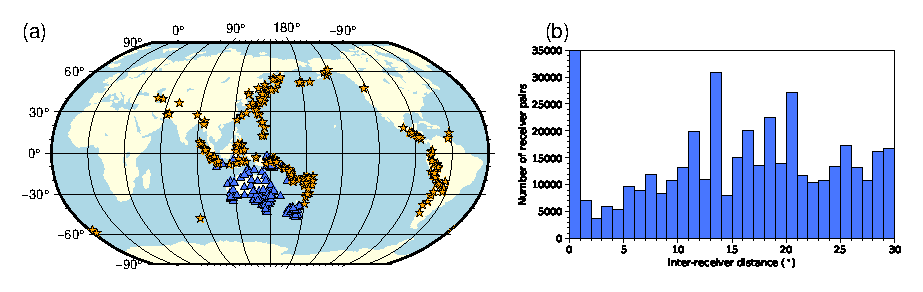
\includegraphics[width=1\linewidth]{figs/correlation_formation/fig_p1_01.pdf}
	\caption[Global events and seismic receivers for analysing coda-correlation's formation]
    {\textbf{(a)} Global distribution of seismic receivers (blue triangles) and events (yellow stars) used in this study. \textbf{(b)} Histogram (receiver pairs) of inter-receiver distances with the bin size of $1^{\circ}$.}
	\label{fig:2.1}
\end{figure}



As shown in Fig. \ref{fig:2.2}a, the correlograms produced for the records in the Australasian region reveal similar patterns to those that utilise global-scale networks  \citep[e.g.,][]{boue_reverberations_2014,pham_earths_2018}. The most prominent features are reminiscent of widely-observed seismic phases: PcP, ScS, and PKIKPPKIKP, and are termed PcP*, ScS*, and I2* following the convention for naming and abbreviation by \citet{tkalcic_shear_2018}. Other features are reminiscent of `exotic seismic phases' such as PKPPcPPKP and PcPPKPPcPPKP that are termed KcK*, and cKcK*. Additionally, there are features such as cS-cP that have no correspondence in seismic wavefield.




% Fig 2
\begin{figure}[!hbt]
	\centering
	\includegraphics[width=1\linewidth]{figs/correlation_formation/fig_p1_02.pdf}
	\caption[Global correlograms built by selecting different receiver pairs]
    {
		Global correlograms constructed by stacking multiple cross-correlation contributions. The most prominent features are labelled following the notation defined by \citet{tkalcic_shear_2018}. \textbf{(a)} All events are used in the stacking. \textbf{(b)} Events are selected for the angle, $\zeta$, smaller than $5^{\circ}$. $\zeta$ is the angle between two great-circle paths that are from the same event to two receivers, respectively. \textbf{(c--f)} Events are selected for the angle, $\zeta$, in ranges of $5-15^{\circ}$, $15-30^{\circ}$, $30-45^{\circ}$, $>45^{\circ}$, respectively.
	}
	\label{fig:2.2}
\end{figure}



\citet{sens-schonfelder_lack_2015} and \citet{poli_analysis_2017} reported that earthquake coda presents unequal energy distribution in different directions and the energy is dominant along great-circle path from an event to a receiver. The lack of equipartitioning hints that coda correlation is dominated by the energy that propagates along the great-circle path. To investigate that, we first construct a global correlogram consisting of all $M_W\geq6.8$ events (Fig. \ref{fig:2.2}a). We then experiment with selecting subsets of those events chosen with respect to event-receiver geometries. We first calculate the angle, $\zeta$, between two great-circle paths defined by an event and two different receivers. If $\zeta$ is $0^{\circ}$, the event and receivers are perfectly aligned and in the same great-circle plane. $\zeta$ can approach $90^{\circ}$ for some events given a pair of receivers, and we expect to see a strong dependence of coda correlation features on it. Figs. \ref{fig:2.2}b--f show the coda correlograms for varying ranges of $\zeta$. Coda-correlation features are clearly prominent when $\zeta$ is close to $0^{\circ}$. The subset of events that satisfy $\zeta$ < $5^{\circ}$ (Fig. \ref{fig:2.2}b) is sufficient to reproduce all coda correlation features (e.g. ScS*, I2*, and cS-cP) seen in the global correlation stack using all events (Fig. \ref{fig:2.2}a). The same is somewhat true for $\zeta$ in the range $5-15^{\circ}$ (Fig. \ref{fig:2.2}c), although some features are significantly diminished in comparison with those in Figs. \ref{fig:2.2}a,b. In contrast, using the events with larger azimuth difference (away from the great-circle plane) results in correlograms with deteriorating correlation features (Figs. \ref{fig:2.2}d,f). In short, when using 3-D global stacks, only those in the great-circle plane constructively contribute to the formation of coda correlation features.


The main result obtained above and demonstrated in Fig. \ref{fig:2.2} narrows the search range to determine the constructive contributions to coda correlation's formation. That is the first stage in resolving coda correlation's formation mechanism. Then, in the second stage, we further determine the exact constructive contributions. The two-stage analysis might seem like reducing a 3-D problem to a 2-D problem. However, it is simply a way to determine the formation of coda correlation features.


To further determine the exact constructive contributions to coda correlation's formation, we therefore focus on earthquake-coda energy in the great-circle plane. We avoid non-contributing energy that is off the great-circle plane by setting an upper limit of $5^{\circ}$ for the angle $\zeta$.



\section{Separation of Contributions to Coda Correlation}\label{sec:theo_sc}

We aim at separating and determining seismic waves in earthquake coda that contribute to coda-correlation features. To achieve this goal, we conduct a temporal variation analysis to determine the timing and energy of individual contributions to each coda correlation feature and an identification analysis to determine seismic waves for each contribution.

\subsection{Temporal variation analysis}\label{subsec:theo_sc_temp}

In coda correlation, interactions between different parts of the earthquake-coda wavefield are manifold. Given the earthquake-coda time-interval, wave propagation through Earth's interior evolves significantly. Moving time windows can explicitly separate different parts of earthquake coda. We use a relatively short moving time window of 100 s with 1 s overlap to calculate coda correlations. The 100 s is twice as long as 50 s, the lowest cut-off frequency of the bandpass filter, as required by the Nyquist-Shannon sampling theorem. This is significantly different from previous studies that use hourly time windows to investigate the optimal time window that produces prominent coda correlation features \citep[e.g.,][]{lin_seismic_2013} or temporal development of a correlation wavefield \citep[e.g.,][]{poli_analysis_2017,kennett_evolution_2018}.



Although earthquake coda from 3 hr after event origin time is used  \citep[e.g.,][]{lin_seismic_2013,pham_earths_2018}, we select earthquake coda in 1--9 hr after event's origin in order to answer why the emergence of coda-correlation features is favoured by the late earthquake coda starting 3 hr after event's origin.




We select the correlation feature I2* at inter-receiver distance of $5^{\circ}$ for its robustness and signal prominence. This feature is reminiscent of PKIKPPKIKP phase in seismic wavefield (Fig. \ref{fig:2.3}a). I2* exists in the small inter-receiver distances and is well formed and pronounced for local-scale network settings. Additionally, I2* has been used as a probe of the Earth's inner core structure \citep[e.g.,][]{huang_high-resolution_2015,wang_equatorial_2015}.



% Fig 3
\begin{figure}[!hbt]
	\centering
	\includegraphics[width=1\linewidth]{figs/correlation_formation/fig_p1_03.pdf}
	\caption[Ray paths of constituents for correlation features I2* and cS-cP]
    {
		Ray paths that contribute to two coda-correlation features: \textbf{(a)} I2* and \textbf{(b)} cS-cP between a pair of receivers (triangles). P-wave ray path legs are shown with solid lines and S-wave ray path legs with dash lines. Different colours represent rays due to different event locations (stars).
	}
	\label{fig:2.3}
\end{figure}


Fig. \ref{fig:2.4}a shows the temporal variations of I2* using the short time window. To quantify the temporal variations, we calculate the coherence of I2* as a function of time. Following \citet{rawlinson_rapid_2004}, the coherence can be measured by taking the inverse of the sum of the squared residual between a normalised I2* using a 100 s time window and the I2* using 3--9 hr:


\begin{equation}\label{eq:2.1}
    coh(\tau) = \frac{1}{|\text{I2}^*_{3-9\text{hr}}-\text{I2}^*_{100\text{s}}(\tau)|^2},
\end{equation}
\myequations{Measurement of coherence of a correlation constituent}

where the $\tau$ denotes the time from the event's origin. The coherence denotes the similarity between an I2* using a moving 100 s length time window ($\text{I2}^*_{100\text{s}}$) and the prominent I2* in global coda correlograms that are produced by using 3--9 hr after event's origin ($\text{I2}^*_{3-9\text{hr}}$). A relatively large coherence indicates that our chosen time window centred on $\tau$ captures a constructive contribution to I2*, whereas low coherence means that corresponding contributions are minimal. Fig. \ref{fig:2.4}b (orange line) presents the coherence variation with the time $\tau$. The spikes indicate discrete contributions to the formation of I2*. There are fewer coherence spikes in the time interval 1--3 hr than in 3--9 hr.

% Fig 4
\begin{figure}[!hbt]
	\centering
	\includegraphics[width=1\linewidth]{figs/correlation_formation/fig_p1_04.pdf}
	\caption[Separation of the I2* constituents]
    {
		Variations of I2* with respect to the time after the event's origin and separation of I2* constituents. \textbf{(a)} Temporal variations of I2* in the following time windows after events: 1--3 3--5, 5--7 and 7--9 hr (left-hand column) and I2* feature using the coda window of 3--9 hr (right-hand column). \textbf{(b)} Normalised coherence (orange line) and energy (blue line) with respect to the time after the event's origin, the coherence and energy are defined in Eq. \ref{eq:2.1} and \ref{eq:2.2}. \textbf{(c)} Isolated constituents of I2* and their picked correlation times by orange arrows (left), and I2* stack of all contributions (right). Horizontal dashed line shows the resulting correlation time of I2*. Each constituent is identified as a cross-term between two seismic waves.
	}
	\label{fig:2.4}
\end{figure}


Apart from the coherence, energy strength is equally important in investigating contributions. The energy strength of a single contribution can be measured following  \citet{sager_sensitivity_2018}:

\begin{equation}\label{eq:2.2}
    E(\tau) = \frac{1}{2}|\text{I2}^*_{100\text{s}}(\tau)|^2.
\end{equation}
\myequations{Measurement of energy strength of a single correlation constituent}

As shown in Fig. \ref{fig:2.4}b (blue line) the energy is relatively strong and oscillatory in 1--3 hr and gradually decreases with the time $\tau$ and becomes stable in later time windows. Only the contributions with large coherence and relatively strong energy can be constructive contributions to correlation features, while those with small coherence but strong energy will `contaminate' correlation features. Finally, those with weak energy and either small or large coherence are negligible.





We investigate temporal variations of various contributions by combining the measure of coherence and energy. For the time interval of 1--3 hr, most of the contributions present small coherence and oscillatory energy, and there are a few spikes in the coherence plot however corresponding energy is weak. The former would contribute destructively and overwhelm the latter in correlation feature's formation. The observed pattern makes the coda wavefield within 1--3 hr ineffective in contributing I2*. For the time interval of 3--9 hr, more contributions emerge with relatively high coherence and strong energy. They dominate the formation of I2* and suppress phase deformations by incoherent contributions. This time-dependent variation of different contributions explains the effectiveness of the late coda in forming prominent features in correlograms, as suggested in previous studies \citep{lin_seismic_2013,poli_analysis_2017,kennett_evolution_2018}.




\subsection{Identification of coda correlation constituents}\label{subsec:theo_sc_iden}

\revcom{This section has been revised in response to comment \#3 of Examiner \#1.}

\revadd{As shown in Fig. \ref{fig:2.4}b,} we identify constructive correlation contributions (constituents), by matching the time $\tau$ of coherence spikes \revadd{(the time of a spike's emergence from the event's origin)} with the arrival times of transient seismic waves, which can be predicted by the ray theory \citep[e.g.,][]{buland_computation_1983}. We attribute a constituent represented by a spike to the cross-term between two seismic waves. Specifically, a constituent at time $\tau$ is the cross-term between two seismic waves that arrive at $\tau$ and $\tau+t$ after event origin time, respectively, where $t$ is the correlation time of a correlogram feature. Arrival-time predictions depend on event locations, although the dependency is moderate for I2* that presents near-zero slowness features (Fig. \ref{fig:2.2}). In the next section, we further analyse the influence of event locations on the correlation time of \revadd{different constituents and their stacks.}



As shown in Fig. \ref{fig:2.4}c, almost all of constructive contributions are identified as cross-terms between seismic waves that reverberate between the Earth's free surface and the core-mantle boundary (CMB). Contributions are insignificant for seismic waves related to the Moho and upper-mantle discontinuities. As for smaller 3-D heterogeneity, associated scattering effects would be less likely to contribute to the formation of coda correlation. Therefore, coda correlation consists of limited types of constituent that are cross-terms between the deep-Earth phases.

\revadd{The observed predominance of deep-Earth phases agrees with the lack of equipartitioning in the late coda \citep{sens-schonfelder_lack_2015,poli_analysis_2017}. These discrete constituents of coda correlation could be considered observational proof of the conjecture that the correlation wavefield is formed by interferences between body waves \citep{pham_earths_2018}.}\revcom{Revised in response to comment \#3 of Examiner \#1.}


Further to analysing I2*, we conduct a similar temporal analysis of another coda-correlation feature: cS-cP and its constituents (Fig. \ref{fig:2.5}). We select cS-cP at inter-receiver distance of $2^{\circ}$. This relatively small inter-receiver distance allows a sufficient number of global events when applying the same great-circle plane requirement ($\zeta<5^{\circ}$). cS-cP displays much faster deterioration than I2* if the same great-circle plane condition is not satisfied (Fig. \ref{fig:2.2}). As shown in Fig. \ref{fig:2.5}, there are discrete contributions to cS-cP, identified as cross-terms between reverberated body waves from the Earth's free surface and CMB, and most of the contributions are in the time interval 3--9 hr after event's origin.


% Fig 5
\begin{figure}[!hbt]
	\centering
	\includegraphics[width=1\linewidth]{figs/correlation_formation/fig_p1_05.pdf}
	\caption[Separation of the cS-cP constituents]
    {
		Similar to Fig. \ref{fig:2.4}, but for the coda-correlation feature cS-cP.
	}
	\label{fig:2.5}
\end{figure}


\section{Characteristic of Coda Correlogram From Its Constituents}\label{sec:theo_charc}

We conduct a quantitative analysis in order to enhance practical understanding of coda correlations. Once coda correlation constituents are fully isolated and identified, we can quantify their relationship with the Earth's structure and dependency on event-receiver geometry.

\subsection{Attributes of coda-correlation constituents}\label{subsec:theo_charc_attr}

A notable feature is the temporal fluctuation of separate constituents of I2* or cS-cP (Fig. \ref{fig:2.4}c or \ref{fig:2.5}c). That variation is on the order of 10 s, which is equivalent to a P-wave isotropic velocity anomaly of $\sim$2 per cent in the Earth's inner core that is sampled by I2*. The variation among waveforms is apparent both in amplitude and phase, which means that the contributing constituents have different sensitivities to Earth structure. This can be expected given that each pair of seismic waves, for example those listed in Figs. \ref{fig:2.4}c and \ref{fig:2.5}c, sample the Earth's interior along different paths. Varied focal mechanism and source-time functions are other reasons for the waveform differences among separated constituents, although they generate less significant time variations than the Earth's structure.




The correlation time of coda-correlation constituents and their variations contain information directly dependent on the Earth's structure. Each correlation time corresponds to the time difference between two seismic waves that can be measured by the cross-term between them. That can be quantified as:


\begin{equation}\label{eq:2.3}
    t_{\text{constituent}} = t_{\text{wave}_1}(\boldsymbol{x}_s, \boldsymbol{x}_{r1}; \boldsymbol{m})- t_{\text{wave}_2}(\boldsymbol{x}_s, \boldsymbol{x}_{r2}; \boldsymbol{m}),
\end{equation}
\myequations{Sensitive of a correlation constituent to the Earth's internal structure and receiver locations}

where the correlation time of a correlation constituent $t_{\text{constituent}}$ can be predicted from the time difference between two seismic wave arrival times $t_{\text{wave}_1}(\boldsymbol{x}_s, \boldsymbol{x}_{r1}; \boldsymbol{m})$ and $t_{\text{wave}_2}(\boldsymbol{x}_s, \boldsymbol{x}_{r2}; \boldsymbol{m})$ that depend on the Earth's structure $\boldsymbol{m}$, locations of an event $\boldsymbol{x}_s$, and two receivers $\boldsymbol{x}_{r1}$ and $\boldsymbol{x}_{r2}$.



% Fig 6
\begin{figure}[!hbt]
	\centering
	\includegraphics[width=1\linewidth]{figs/correlation_formation/fig_p1_06.pdf}
	\caption[An `anatomy' of the cross-term I6-I4, one of the I2* constituents]
    {
		An `anatomy' of the cross-term I6-I4, one of I2* constituents. \textbf{(a)} Synthetic distribution of sources (stars) and two fixed receivers (triangles) that are used in analysing characteristics of I6-I4. The ray path of I2 (black line) from one receiver to the other. \textbf{(b)} Ray paths of I6 (blue lines) and I4 (orange lines) from the event at the stationary (the same slowness) point to the two fixed receivers. \textbf{(c)} Variations of I6-I4 cross-term as a function of event locations. The correlogram is created using the distribution of events in (a). Red dash line denotes theoretical arrival-time difference between I6 and I4 based on the ak135 Earth model \citep{kennett_constraints_1995}. \textbf{(d)} Theoretical slowness curves for I4 (solid line) and I6 (dash line). The black dots denote the event location where I4 and I6 have the same slowness and the I6-I4 differential time curve has the curvature of 0.
	}
	\label{fig:2.6}
\end{figure}


We assess that quantification through a synthetic experiment as follows. We use the axisymmetric spectral element method, AxiSEM \citep{nissen-meyer_axisem_2014}, to simulate synthetic coda wavefield for the actual event-receiver geometry settings. In our simulations, we employ a spherically symmetric Earth model ak135  \citep{kennett_constraints_1995}. We use explosive mechanism and Gaussian source time function with a dominant period of 10 s following \citet{pham_earths_2018}. We consider two fixed receivers with a $5^{\circ}$ separation and events distributed globally along the great-circle path defined by the two receivers (Fig. \ref{fig:2.6}a). We choose the cross-term between I6 and I4 phases for our analysis, and we calculate cross-terms for events at different longitudes. We do not consider varied focal mechanisms or source time functions in the simulation to keep the synthetic experiment simple.

As shown in Fig. \ref{fig:2.6}c, the correlation time of cross-term I6-I4 equals the arrival-time difference between I6 and I4 that are predicted using ray theory. Significantly, the cross-term I6-I4 exhibits varied correlation time when events are in different locations (hyperbolic in shape as a function of event longitude). The time variation curve has a saddle-point minimum around which the curvature is nearly flat (Fig. \ref{fig:2.6}c). At the minimum, I6 and I4 have the same slowness and a portion of the ray paths in common (Figs. \ref{fig:2.6}b,d). Only at the point, the differential ray path equals to PKIKPPKIKP between two receivers. This equivalence does not exist for other event locations, and hence there are time variations, waveform distortion, and even the absence of I2* in extreme cases (Fig. \ref{fig:2.6}c). Similar time variations hold for other constituents, for example I8-I6, I10-I8, etc. (Fig. \ref{fig:2.S1}).



Eq. \ref{eq:2.3} denotes a quantitative relationship between coda-correlation and the Earth's structure. Given a model the Earth's internal structure, the correlation time of a coda-correlation constituent can be predicted. Through decreasing the difference between the predictions and observations, an inverse problem can be built towards inverting the Earth's structure.

\revadd{Also, Eq. \ref{eq:2.3} implies that a coda correlation feature and its constituents can be affected by the source mechanisms and energy-release dynamics that shape the seismic waves($\text{wave}_1$ and $\text{wave}_2$). \citet{tkalcic_excitation_2020} and \citet[Chapter \ref{ch:intersrc}]{wang2022inter-src} find out that the thrust- and normal-fault sources are effective for forming many prominent global correlation features because the sources are efficient for radiating deep-travelling energy that are the main contributions to creating the features. In comparison, strike-slip and dip-slip sources are less effective.}
\revcom{Revised in response to comment \#4 of Examiner \#1.}


\subsection{Formation of a coda-correlation feature by many constituents}\label{subsec:theo_charc_form}



The time variations introduced due to event locations have a significant bearing on the formation of coda correlation features. When the time variations around the same slowness point, as shown in Fig. \ref{fig:2.6}c, are nearly zero, the corresponding cross-terms contribute constructively to cross-correlation stacks to produce a stable correlation feature. In contrast, large time variations result in non-constructive contributions whose cross-terms dilute the stacks. We further group events according to their distance to the same slowness point and stack I6-I4 cross-terms to produce I2*. As shown in Fig. \ref{fig:2.7}, the stacked I2* has a relatively stable timing if we limit events to only those within $10^{\circ}$ around the same slowness point. There is a severe time shift if all events on global scale are used: this results in a time shift of I2* up to $\sim$4 s. Such a time shift is equivalent to $\sim$1 per cent P-wave isotropic-velocity perturbation of the entire inner core sampled by I2*.



Furthermore, the time variations due to event locations are significantly different among different I2* constituents, which is illustrated in Fig. \ref{fig:2.8}. The cross-terms between seismic waves in late earthquake-coda (3 hr after the event origin time) present much smaller time variation ranges than those formed by the seismic waves in early time windows (1--3 hr from the event origin time). For example, I6-I4 presents time variation ranging up to $\sim$61 s due to event locations, whereas I24-I22 has much smaller time variation of $\sim$6 s. That pronounced difference explains why the published late-coda correlograms favour the emergence of coda-correlation features  \citep[e.g.,][]{lin_seismic_2013,poli_analysis_2017}. Namely, only for the late coda, body-wave cross-terms exhibit less location-dependent time variations, and hence their stack can effectively produce stable correlation features.

% FIg 7
\begin{figure}[!hbt]
	\centering
	\includegraphics[width=1\linewidth]{figs/correlation_formation/fig_p1_07.pdf}
	\caption[Variation of the I2* due to different selections of events]
    {
		Variation of correlation stacks due to different selections of events. Colours denote different selections of events around the stationary (the same slowness) point for the correlogram stacking. The black rectangle shows the time variation of $\sim$4 s for I2* in the cross-correlation maxima for different selections of event zones around the stationary point expressed in $^{\circ}$.
	}
	\label{fig:2.7}
\end{figure}


% FIg 8
\begin{figure}[!hbt]
	\centering
	\includegraphics[width=1\linewidth]{figs/correlation_formation/fig_p1_08.pdf}
	\caption[Variation of individual I2* constituent due to event locations]
    {
		\textbf{(a)} Differential correlation time curves for different I2* constituents, with respect to event locations. The colour dots denote the events located in the stationary (the same slowness) points for corresponding cross-terms. \textbf{(b)} Correlation-time variation maxima for different cross-terms due to the selection of events located away from the stationary points. Time variation maxima significantly decrease for cross-terms of higher reverberated body waves.
	}
	\label{fig:2.8}
\end{figure}




In terms of comparing the 2-D and 3-D effects, the cross-terms for 3-D Earth include both those in the great-circle plane and those outside the great-circle plane. As demonstrated in Section \ref{sec:theo_cc}, the former mainly contribute to the formation of coda-correlation features, while the latter do not contribute significantly. Therefore, stacking of all cross-terms for 3-D Earth becomes well represented by a synthetic experiment reduced to the great-circle plane configuration. The only difference is that the global-scale stacks for 3-D Earth include more non-contributing cross-terms of seismic waves that propagate outside the great-circle plane.

The relationship between cross-terms of seismic waves and the Earth's structure always varies significantly with respect to event locations, although cross-terms presents small time variations when late coda is used. As shown in Fig. \ref{fig:2.9}, from different events, ray paths are completely different for cross-terms between seismic waves that are either in early coda such as I6-I4 or in the late coda such as I22-I20 and I28-I26, although the latter present much smaller time variations.


% FIg 9
\begin{figure}[!hbt]
	\centering
	\includegraphics[width=0.96\linewidth]{figs/correlation_formation/fig_p1_09.pdf}
	\caption[Ray paths of different I2* constituents]
    {
		Ray paths of different I2* constituents. \textbf{(a)} Ray paths for cross-term I6-I4 for an event in the stationary (the same slowness) point (left-hand column) and for two events away from the stationary points (middle and right-hand columns). Time difference in seconds for each event is shown above each cross-section. \textbf{(b--d)} similar to (a) but for cross-terms of I14-I12, I22-I20 and I28-I26.
	}
	\label{fig:2.9}
\end{figure}



Therefore, to produce stable coda-correlation features, we can either use the late coda, as suggested in previous studies \citep[e.g.,][]{lin_seismic_2013,poli_analysis_2017}  or carefully select events and cross-terms in early time windows. If using the late coda without event selections, it is important to recognise the variation of cross-term ray paths, although the associated correlation time can be nearly invariant. A good example is one of the I2* constituents, I28-I26, whose time variation is $\sim$5 s in maximum (Fig. \ref{fig:2.8}). Fig. \ref{fig:2.9} shows the ray paths for some of the I2* constituents for the events located in stationary points (left-hand column) and randomly selected event locations (right-hand columns). For example, I6-I4 is shown in Fig. \ref{fig:2.9}a, and I28-I26 is shown in  Fig. \ref{fig:2.9}d. Even if the event is located in the corresponding stationary point, the sampled volume of the Earth's interior increases considerably for I28-I26 in comparison to I6-I4, and we lose the lateral resolution of the deep earth.


\section{Discussions and Conclusions}

We have shown that a coda correlation feature consists of discrete and time-dependent contributions. Notably, most of these contributions reside in the late coda, 3 hr after the origin time and later, while the early time-interval presents many incoherent constituents with varying energy. There are quite a few coherent contributions in 1--3 hr, though their energy is relatively weaker than the energy of incoherent ones. Specifically designed short-time windows based on temporal analysis could remove incoherent contributions and their `contamination' effects. This makes it possible to promote coda correlations to an early time interval.

Our quantitative separation and identification procedures confirm that coda correlations are dominated by cross-terms between seismic phases that are sensitive to deep-Earth structure and propagate in the great-circle plane. Those seismic phases stem from reverberations between the Earth's free surface and the CMB, whereas the interactions with minor discontinuities and lateral heterogeneity are insignificant. This represents an observational proof to the mathematical conjecture suggested recently  \citep{pham_earths_2018,tkalcic_shear_2018,kennett_nature_2018}. Apart from that, it indicates that the late-coda wavefield is not diffuse, a concept equivalent to the unequal energy distribution \citep{maeda_constituents_2006,sens-schonfelder_lack_2015,poli_analysis_2017}. Instead, the late coda is predominated by deep-Earth phases and hence nearly zero-slowness features (e.g. I2*) significantly exceed large slowness features (e.g. P*) in global coda correlograms \citep[][;Fig. \ref{fig:2.2}]{boue_reverberations_2014,pham_earths_2018}.

There are significant differences between the cross-correlation of late earthquake-coda and the cross-correlation of a diffuse wavefield (e.g., ambient noise wavefield) in which cross-correlation features are equivalent to reconstructed seismic waves. In a diffuse wavefield, energy is equally distributed in different directions. `Non-causal' cross-terms in individual cross-correlation functions destructively interfere and cancel each other in stacking, and hence cross-correlation stacks converge to reconstructed seismic waves \citep[e.g.,][]{snieder_cancellation_2008,snieder_cancellation_2010}. However, in late earthquake-coda, cross-correlation functions are dominated by cross-terms of deep-Earth phases. Stacking them not only does not cancel them out but results in `non-causal' features, such as cS-cP.



In coda correlation wavefield, seismic-wave cross-terms present different time variation with respect to the selection of events. Cross-terms of seismic waves in late coda time windows present nearly invariant correlation time and hence their stacking results in constructive interference to produce stable correlation features. This explains the increasing number of contributions after 3 hr from the event origin time (Figs. \ref{fig:2.4}c and \ref{fig:2.5}c). The correlation time of those cross-terms presents less sensitivity to the event locations, and hence they are quite stable when global events are used without selection. In contrast, cross-terms from early time windows present relatively large time variations.



The insensitivity to event locations in the late coda has practical implications. A stable emergence of coda-correlation features does not necessarily mean a stable reconstruction of body waves. The stable emergence results from the nearly invariant timing of cross-terms. However, the ray paths vary significantly with event locations  Fig. \ref{fig:2.9}. Therefore, cautions must be exercised in all interpretations or utilisations, and it is necessary to investigate ray path variations related to event locations.



% Fig S1
\begin{figure}[!hbt]
	\centering
	\includegraphics[width=1\linewidth]{figs/correlation_formation/fig_S01.png}
	\caption[Theoretical arrival-time and slowness curves for different I2* constituents]
    {
		\textbf{(a--f)} Theoretical arrival-time curves and differential time curves for cross-terms of I6-I4, I10-I8, I14-I12, I18-I16, I22-I20, and I26-I24, respectively. \textbf{(g--l)} Theoretical slowness curves for cross-terms of I6-I4, I10-I8, I14-I12, I18-I16, I22-I20, and I26-I24, respectively. The black dots denote the stationary (the same slowness) points. 
	}
	\label{fig:2.S1}
\end{figure}


Coda correlation tomography is feasible based on our comprehensive analysis. The sensitivity kernel for tomography can be constructed by relating each of the identified constituents to the Earth's structure based on Eq. \ref{eq:2.3}. With informed choice of events, the differential sensitivity between two seismic waves can be obtained. The tomography kernel consists of many differential sensitivities, each of which corresponds to an identified seismic-wave cross-term. This approach is similar to building differential kernels  \citep[e.g.,][]{calvet_traveltime_2005,ruigrok_scanning_2012}. The sensitivity and accuracy can be evaluated with either ray-approximation-based routines \citep[e.g.,][]{cerveny_seismic_2005} or finite-frequency methods \citep[e.g.,][]{marquering_three-dimensional_1999,dahlen_frechet_2000,hung_frechet_2000}. The kernel construction framework is different from the conventional one in which inter-receiver cross-correlation stacks are treated as Green's function. In the Green's function approach, all of the available events and the full coda time window are used. In contrast, the new approach precisely relates each constituent of correlogram features to the Earth's structure. Also, our analyses show that there are multiple constituents for each feature in correlograms. Therefore, even a single feature in correlograms may provide a well-posed inference on the Earth's structure.

Finally, the separation and identification of constituents are labour-intensive steps. Some constituents cannot be separated. For example, PcSPKIKP-PcS and PcSPKIKP-ScP possess nearly identical arrival time. They cannot be separated from each other though they have fundamentally different sensitivities to the Earth's structure. It is necessary to avoid this kind of indistinguishable cross-terms and select other unambiguous cross-terms for accurate tomographic inference. We can use short-time windows around the arrival times of the phases we select, for instance PKIKPPKIKP and PKIKP, and calculate the cross-term between them \citep[][Chapter \ref{ch:tomo}]{wang2020seismictomo}. Also, the computation and visualisation requirements are significant due to the short moving time windows, and modern high-performance computation facilities are necessary. Despite these obstacles, the study presented here is a foundation for a quantitative utilisation of coda correlations, and we look forward to further improvements for standard and target-oriented approaches in different seismological problems.

\section*{Acknowledgements}

The computation and visualisation were performed on the ANU Terrawulf cluster, a computation facility developed with support from the AuScope initiative. Waveform data used in this study are retrieved from \href{https://doi.org/10.7914/SN/II}{IRIS/IDA Seismic Network } operated by Scripps Institution of Oceanography (SIO)/IRIS (\citeyear{scripps_institution_of_oceanography_global_1986}), \href{(https://doi.org/10.7914/SN/IU}{Global Seismograph Network} operated by  Albuquerque Seismological Laboratory (ASL)/USGS (\citeyear{albuquerque_seismological_laboratoryusgs_global_1988}), and \href{(https://doi.org/10.7914/SN/GA}{Australian National Seismograph Network} operated by Geoscience Australia (GA).




\include{Chapters/Chapter03}
\include{Chapters/Chapter04}
\include{Chapters/Chapter04-SI}
\include{Chapters/Chapter05}
\include{Chapters/Chapter06-NA}
\include{Chapters/Chapter06-NA-SI}
\input{Chapters/Chapter06-NA-SI-FIGS}
%\include{Chapters/Chapter06}
%\include{Chapters/Chapter06-SI}
%\include{Chapters/Chapter06-SI-FIGS}
\include{Chapters/Chapter07}
%

%----------------------------------------------------------------------------------------
%	BIBLIOGRAPHY
%----------------------------------------------------------------------------------------
%Use the executable file provide here to clean-up Mendeley generated bib files
%https://ramblingacademic.com/2016/06/19/fixing-bibtex-files-mendeley/ 
% or the python script at https://tex.stackexchange.com/questions/286261/incompatible-month-formats-between-biblatex-and-mendeley

\printbibliography[heading=bibintoc]

%----------------------------------------------------------------------------------------
%----------------------------------------------------------------------------------------
%	THESIS CONTENT - APPENDICES
%----------------------------------------------------------------------------------------

\appendix % Cue to tell LaTeX that the following "chapters" are Appendices

% Include the appendices of the thesis as separate files from the Appendices folder
% Uncomment the lines as you write the Appendices

%\include{Appendices/AppendixA}
%\include{Appendices/AppendixB}
%\include{Appendices/AppendixC}

\clearpage

%\listoffixmes

%----------------------------------------------------------------------------------------
%----------------------------------------------------------------------------------------

\end{document}  